% ======================================================================
% Results, four sections, built around the two halves of the title.
%   2.1 the record: one identity across 55 databases
%   2.2 what a forward screen inherits: the labels, then the pool, then what
%       the integration itself added to the pool
%   2.3 probing the limit: completing the property layer  <- models pending
%   2.4 inverse: judging the novelty claimed by inverse design  <- audit pending
% Implementation detail lives in Methods and the Supplementary Information.
% ======================================================================
\section{Results}

\subsection{One record from 55 databases}
\label{sec:index}

Making 55 databases comparable comes down to one decision, taken once per
incoming record: is this crystal already in the corpus? We settle it on the
structure rather than on the label. Each record is matched first on a
cross-database identifier the source is entitled to assert, then on a structural
fingerprint, and never on the chemical formula, which polymorphs share
(Fig.~\ref{fig:architecture}a; Methods). A record that matches nothing is
admitted rather than discarded, and every value it carries keeps the source, the
native record and the method behind it. That second choice has a consequence this
section measures: because an admitted record joins the criterion applied to the
next, what results is not a merge of 55 databases but a corpus that extends the
substrate it recognises them against.

The corpus so assembled holds 14{,}590{,}485 distinct crystal structures, of
which 357{,}127 are experimental and 14{,}233{,}358 are computational candidates.
On that pool sit 131{,}824{,}881 property values spanning 166 properties,
1{,}198{,}897 stored spectra and 21{,}543{,}633 references recording which
database contains which crystal.

The contributors are extremely unequal, spanning 5.7 orders of magnitude, with
the largest supplying 46.0\% of all values and 30 of the 55 supplying fewer than
$10^5$ each (Fig.~\ref{fig:architecture}b). The two ends of that distribution do
different work: the large general-purpose databases determine how much of the
pool carries any property at all, while the small specialised libraries determine
how many distinct properties exist to carry
\cite{haastrup2018c2db,zhou20192dmatpedia,zhang2019catalogue} \textemdash{} the
most property-diverse contributor supplies 61 of the 166 properties, the largest
supplies 10.

The corpus is considerably larger than the pool it started from, and the
difference is exactly the records that matched nothing
(Fig.~\ref{fig:architecture}c). The deduplicated starting pool held 8{,}225{,}138
structures, and admission added 6{,}365{,}347 more, a growth of 77.4\%. Of the
21{,}543{,}633 references, 6{,}784{,}564 were resolved by record identifier,
8{,}294{,}560 by structural fingerprint alone, and the remainder record a
database's own entry (Fig.~\ref{fig:architecture}d). The two matched routes are
not interchangeable: identifier matching is exact but available only where a
database publishes a cross-reference it owns, while fingerprint matching is
available everywhere but has a domain of validity.

That domain has an edge, and it is worth stating before any conclusion is drawn
from the corpus. Enumerated framework libraries are generated by decorating a
small number of parent topologies, so sibling entries are identical in everything
a bonding-graph fingerprint reads and more than $10^5$ distinct hypothetical
frameworks would collapse onto a few hundred pool materials. Such libraries are
detected at the level of the source rather than the record and admitted under a
composite key, and the boundary of validity this establishes is stated in
Supplementary Note~\ref{si-note:fingerprint}.

\begin{figure}[p]
  \centering
  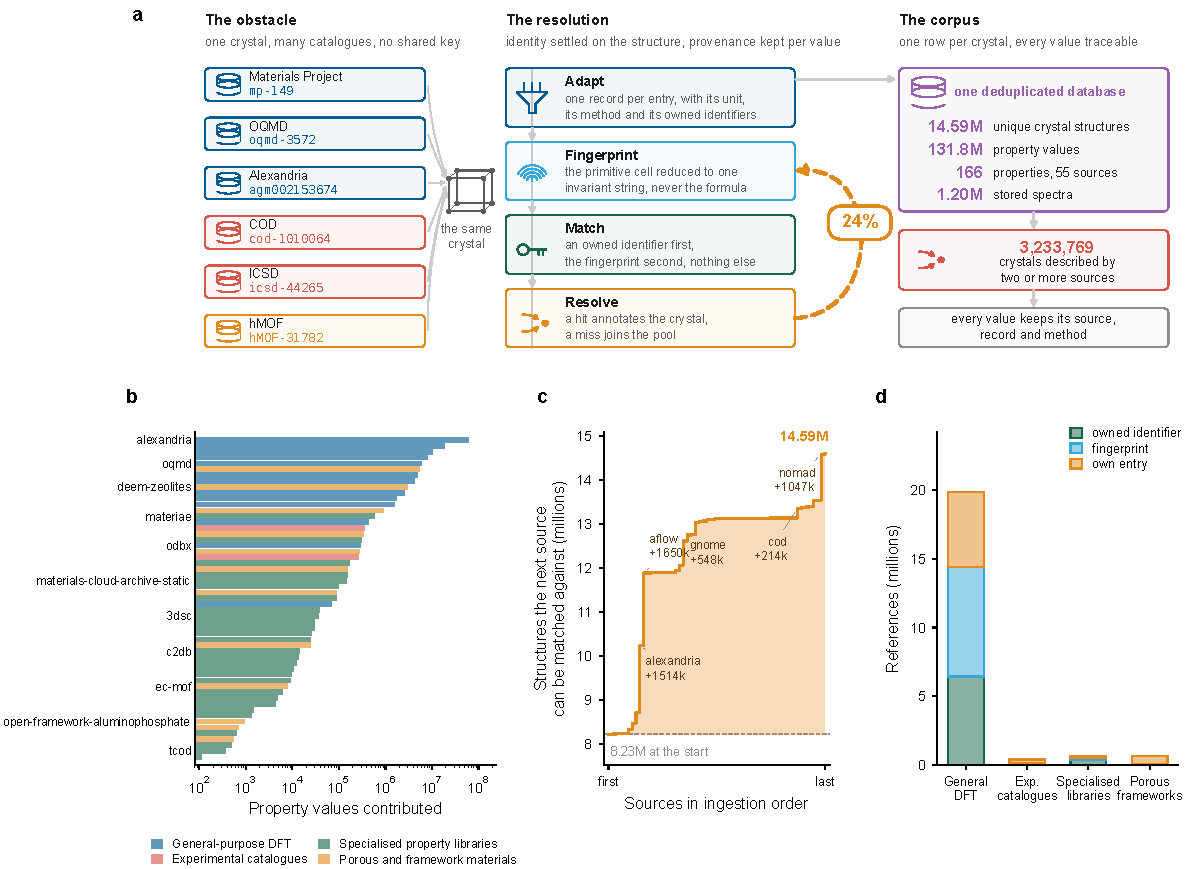
\includegraphics[width=0.99\textwidth]{figs/fig1_architecture.pdf}
  \caption{\textbf{Making the source databases comparable at the level of the
  crystal.}
  \textbf{a},~The obstacle and the resolution. Each database labels the same
  arrangement of atoms with its own accession number, and no key relates them.
  Every incoming record is reduced to a structural fingerprint and matched first
  on a cross-database identifier the source is entitled to assert, second on that
  fingerprint, never on the chemical formula. The dashed loop is the mechanism
  that makes the corpus self-evolving: a record matching nothing is admitted, and
  its fingerprint re-enters the matcher, so each source is matched against a
  larger pool than the one before it. The figure on the loop is the percentage of
  all matches that land on a crystal admitted this way. The right column reports
  what the assembled corpus holds.
  \textbf{b},~Property values contributed by each database on a logarithmic axis,
  coloured by family, with labels at regular intervals through the ranking.
  \textbf{c},~The loop of \textbf{a}, measured. Each step is one source's
  admissions entering the match map, so the height at any point is the number of
  crystals the next source could be matched against. The largest single
  contributions are labelled.
  \textbf{d},~How the references were resolved, grouped by database family: by an
  identifier the source owns, by structural fingerprint, or as a record that the
  database contains the structure itself.}
  \label{fig:architecture}
\end{figure}

A structure admitted from one database becomes recognisable to every database
that follows, because its fingerprint and identifiers join the matching substrate
as it is admitted. The corpus therefore does not merely accumulate: the criterion
by which it recognises the next record is itself a product of the records already
ingested, and it is by this mechanism that the database keeps itself current as
sources publish new versions and new sources appear. The effect is measurable. Of
the 15{,}079{,}124 references resolved by matching, 3{,}676{,}707, or 24.4\%,
land on a crystal that was absent from the starting pool and was admitted during
assembly (Fig.~\ref{fig:redundancy}c). Those links do not exist in a construction
that matches every database against a fixed reference. The figure is a property
of the assembly rather than of the sources, since a different ingestion order
would distribute it differently between them, and it is a lower bound on what a
frozen reference would have missed rather than a measure of quality. What it
establishes is that such links exist at all, and how much of the record they
reach.

The effect is ordered by ingestion time and by chemical distance from the
starting pool. AFLOW, ingested about ninety minutes after Alexandria contributed
1{,}514{,}488 structures, resolved 47.7\% of its 1{,}401{,}895 matches onto
crystals admitted during assembly. The JARVIS tight-binding set, whose fitting
geometries are deliberately non-equilibrium and largely absent from the starting
pool, reached 67.6\%. The framework libraries show the effect in its purest form:
CoRE MOF, ingested last among them, resolved 99.5\% of its matches onto
frameworks contributed by four earlier libraries. NOMAD
\cite{draxl2019nomad}, the last source ingested of the 55 and so the one matched
against the largest substrate, resolved 56.1\% of its 3{,}168{,}530 matches onto
crystals the starting pool did not contain, and contributed 1{,}047{,}208
structures of its own that now form part of the criterion applied to whatever is
ingested next. Databases whose chemistry the starting pool already covered show
the converse, at or near zero.

The practical consequence is that the marginal value of adding a database is not
confined to the values it brings. CoRE MOF contributed 155{,}488 experimental
porosity measurements, and the reason 99.5\% of them landed on an existing
crystal rather than forming an isolated set of new ones is that earlier libraries
had already put those frameworks in the pool. Assembled against a frozen
reference, the same measurements would have arrived as an unconnected island, and
the corpus would have to be rebuilt from the beginning to connect them.

\subsection{What a forward screen inherits}
\label{sec:inherits}

A forward screen inherits two things from whichever database it loads: the labels
it trains on and the pool it ranks. Neither is a property of the method, and
neither can be measured from inside a single database, because each is a property
of the record as a whole. Measured on the resolved union, both are worse than the
database a campaign loads is able to report. Where two independent sources
describe the same crystal they disagree by more than the margin conventionally
used to decide whether a compound is stable; and almost a quarter of the labelled
record is unavailable from any single provider. This section establishes the two
in that order.

Measuring the labels begins with how much of the record is one crystal counted
several times, which no member source can answer and a formula-level join would
answer wrongly in both directions. Of the 13{,}902{,}836 structures carrying at
least one reference, 3{,}233{,}769 carry two or more
(Fig.~\ref{fig:redundancy}a), and the distribution falls steeply while reaching
far: 2{,}395{,}350 crystals are described by exactly two databases, 568{,}507 by
three, 2{,}416 by thirteen and two by 25. Redundancy is concentrated where the
field has concentrated its effort. The largest single overlap holds
1{,}672{,}167 shared crystals, and the eight largest are all between
general-purpose density functional theory repositories
(Fig.~\ref{fig:redundancy}b); the enumerated framework libraries sit outside this
entirely, sharing almost nothing with the general-purpose repositories or with
one another, so the blank rows of the overlap matrix record where effort has gone
rather than a gap in the corpus. These are the numbers a federated query cannot
report and a formula-level join would misstate in both directions, and they bound
what any cross-database evaluation can claim: for the largest overlapping pairs,
a model trained on one repository and tested on another is tested on hundreds of
thousands of crystals it has already seen, unless the split is taken over
structures.

\begin{figure}[p]
  \centering
  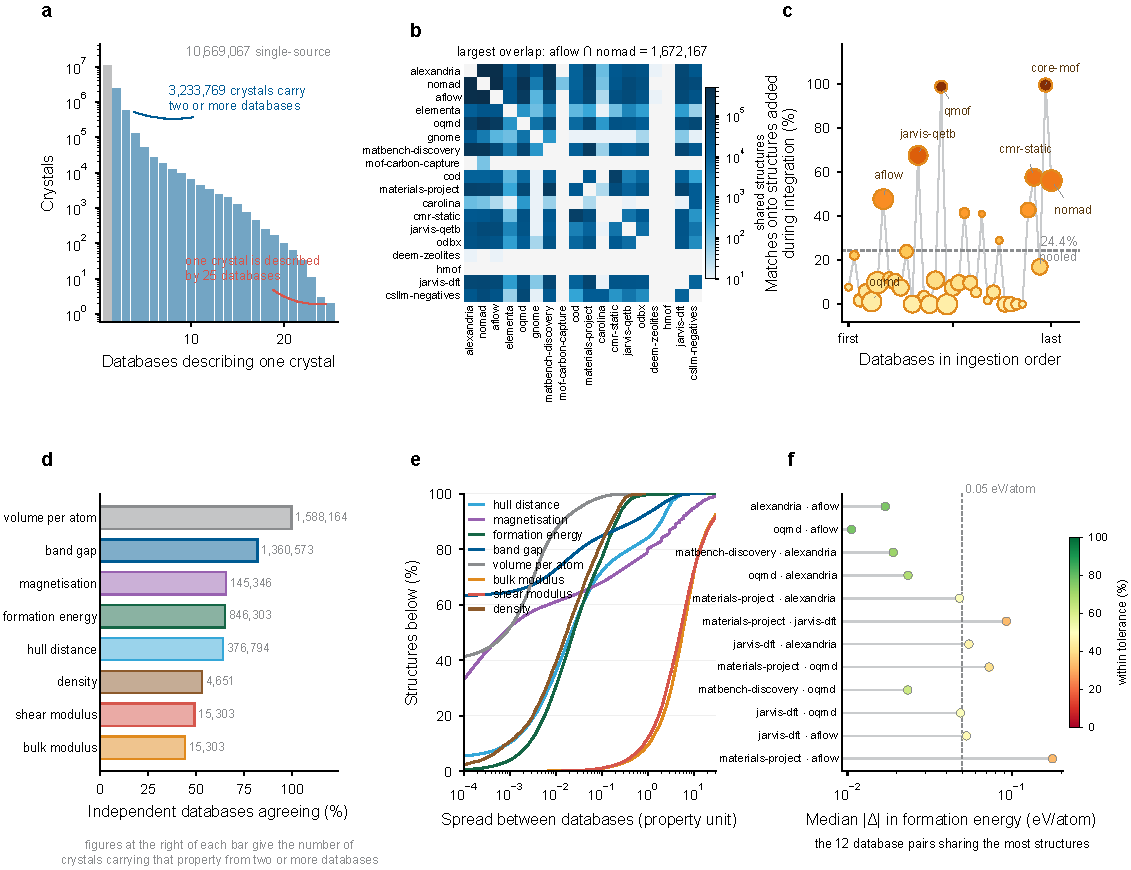
\includegraphics[width=0.99\textwidth]{figs/fig2_redundancy.pdf}
  \caption{\textbf{Redundancy between databases, and whether the duplicates
  agree.}
  \textbf{a},~Number of databases describing one crystal. Grey marks the crystals
  held by a single database, blue those held by two or more.
  \textbf{b},~Shared crystals between the databases annotating the most
  structures, on a logarithmic colour scale. An empty cell marks a pair with no
  crystal in common rather than missing data.
  \textbf{c},~The growing recognition substrate. For each database, in ingestion
  order, the fraction of its matches landing on a crystal absent from the
  starting pool and admitted during assembly. Marker area scales with the number
  of matches, and the dashed line is the value pooled over all databases.
  \textbf{d},~For each comparable property, the fraction of multi-source crystals
  whose independent values fall within the tolerance stated in
  Supplementary Note~\ref{si-note:agreement}. The figure beside each bar is the
  number of crystals carrying that property from two or more databases at one
  level of theory.
  \textbf{e},~Cumulative distribution of the spread between databases, in the
  property's own unit for energies, magnetisation and moduli and as a relative
  difference for density and volume per atom.
  \textbf{f},~Median absolute difference in formation energy for the database
  pairs sharing the most crystals, coloured by the fraction agreeing within the
  tolerance marked by the dashed line.}
  \label{fig:redundancy}
\end{figure}

Redundancy is only interesting if the redundant copies can be compared, and they
can be compared here only because every value kept the method that produced it.
Every method string is collapsed to a level of theory, and two databases are held
against one another only where they answer the same question: a semilocal value
is compared with a semilocal value, a measurement with a measurement, and a pair
that meets only across that boundary is not compared at all
(Fig.~\ref{fig:redundancy}d--f; Supplementary Note~\ref{si-note:agreement}).
The comparison is possible on a large sample: 1{,}360{,}573 crystals carry a band
gap from two or more databases at one level of theory, 846{,}303 a formation
energy, 376{,}794 a hull distance, 145{,}346 a magnetisation and 15{,}303 a bulk
modulus. Concordance falls as the quantity becomes harder to compute. Within
50~meV, 82.1\% of shared band gaps agree. Within 50~meV\,atom$^{-1}$, 65.3\% of
formation energies and 64.2\% of hull distances do, and within 5~GPa, 44.3\% of
bulk moduli and 49.3\% of shear moduli do.

The tail matters more than the median. The tenth of shared formation energies
that agree least differ by more than 205~meV\,atom$^{-1}$
(Fig.~\ref{fig:redundancy}e), which is several times the hull-distance margins
conventionally used to call a compound stable
\cite{sun2016thermodynamic,bartel2020critical}. Whether a candidate passes such a
filter can therefore depend on which database supplied its energy, and in a
corpus without structural identity that dependence is not merely unquantified but
unobservable. This is the first of the section's two results.

It survives three checks, and each sharpens it rather than softening it. The
first is that agreement between two databases is not evidence of independence, so
the concordant fraction quoted above overstates it. Resolving the comparison by
pair separates two regimes that a single agreement figure would merge
(Fig.~\ref{fig:redundancy}f). Some pairs agree almost exactly.
Two of the largest repositories share 138{,}959 crystals whose band gaps have a
median absolute difference of exactly zero and agree within tolerance for 92.3\%
of them. That is not independent confirmation but the signature of shared
provenance, two datasets carrying one underlying calculation, and reading it as
corroboration would invert its meaning. Other pairs disagree systematically. For
formation energy the median signed difference between the Materials Project and
JARVIS-DFT is $+70.7$~meV\,atom$^{-1}$ against a median absolute difference of
92.7~meV\,atom$^{-1}$, so nearly all of the disagreement carries one sign. The
corresponding figures are $+171$ against 177~meV\,atom$^{-1}$ for the Materials
Project against AFLOW. Pearson correlations across these pairs remain between
0.85 and 0.99, so what separates the databases is an offset and a scale rather
than noise. This is precisely the structure that merging columns by name would
absorb without trace, and precisely the structure a model trained on the merged
column would learn as if it were physics.

The second check is that the offsets are not a failure of the underlying theory,
so they will not be removed by better software. Forty independent
implementations of density
functional theory, run on the same systems with the same functional, agree on the
equation of state to well within the differences reported here
\cite{lejaeghere2016reproducibility}. What separates two databases is therefore
not the solver but the accumulation of choices each provider makes around it, the
pseudopotentials, the functional, the convergence criteria and the elemental or
anionic corrections applied afterwards, none of which is visible in a column of
numbers labelled formation energy. The reproducibility of the theory bounds what
a careful user could hope for; the disagreement measured here is what a user
actually receives.

The third check is that the disagreement is not an artefact of comparing
different quantities, and the method strings are what make it checkable. A
further 24{,}380 crystals carry a formation energy from two databases that worked
at different levels of theory; they are deliberately left uncompared, because the
difference between a tight-binding and a semilocal energy is not a disagreement.
For density the excluded overlap is the larger part of it, 37{,}770 crystals
against 4{,}651 compared, since the experimental catalogues and the computed
repositories are not reporting the same quantity. Excluding these pairs lowers the
measured disagreement rather than raising it, so the figures above are what
remains after the comparison has been made fair. A union that merged the columns
by name would have reported every excluded pair as a discrepancy instead.

Measuring the disagreement is not all the comparison is good for. It also
identifies what no single-source check would question, at two scales. At the scale of the value,
1{,}161 of the shared elastic moduli lie outside any physically plausible range,
being negative or above 1000~GPa, the largest reaching
$1.4\times10^{13}$~GPa. These are unconverged elastic-tensor fits published as
they stand, and in isolation each is simply a number in a column; set against a
partner value on the same crystal, each is immediately identifiable. At the scale
of the column, one source that carries several levels of theory for the same
crystal turns out to supply one band-gap column that tracks an independent
repository closely and another, at a different level, that correlates with it at
$r=0.09$ because it reports almost every crystal as a metal
(Supplementary Note~\ref{si-note:agreement}). From inside that column the result
reads as a list of metals and nothing marks it as wrong. It is legible here only
because the same crystals carry an independent value, and separable from the
usable column beside it only because the level of theory travelled with every
number.

The pool is the second inheritance, and the question it raises is how much of it
carries any label at all. The answer is: very little, and what there is was not
distributed by importance, nor even by cost. Of the 166 properties in the registry, 151 carry at least one value. Treating the pool and
those 151 properties as a matrix gives 2{,}203{,}163{,}235 cells, of which
99{,}493{,}466 are occupied, so the matrix is 4.52\% full
(Fig.~\ref{fig:landscape}a). Occupancy is extremely uneven: nine properties cover
more than 40\% of the pool, while 97 of the 151 cover less than 1\% and 58 cover
less than 0.1\% (Supplementary Table~\ref{si-tab:properties}). Half of all
crystals carry at most seven of the 151 properties (Fig.~\ref{fig:landscape}c).

\begin{figure}[p]
  \centering
  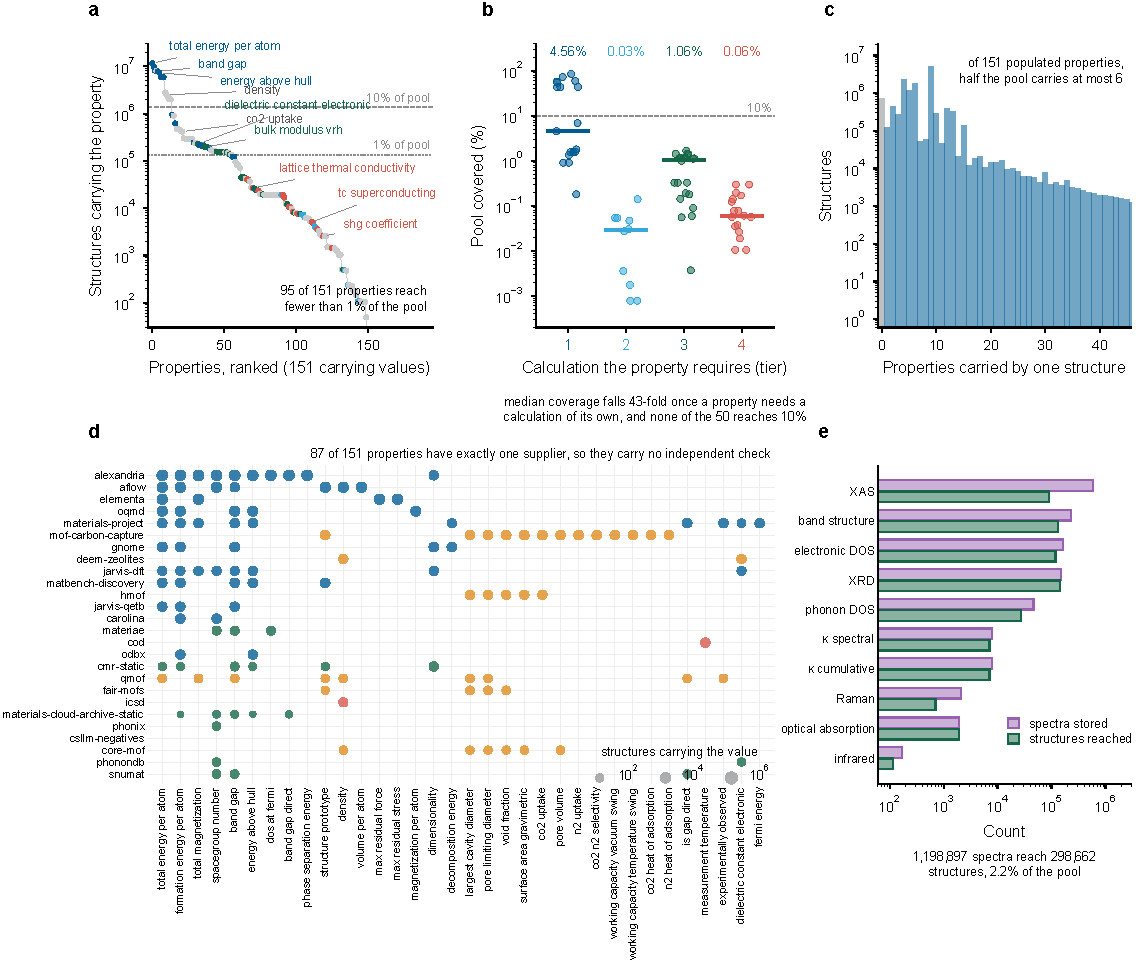
\includegraphics[width=0.99\textwidth]{figs/fig3_landscape.pdf}
  \caption{\textbf{What the corpus contains, and what it does not.}
  \textbf{a},~Every property carrying at least one value, ranked by the number of
  crystals that carry it. Colour marks the calculation tier assigned in
  \textbf{b}. Grey marks properties outside that classification, whose domain is
  a single material family. The horizontal lines mark the stated fractions of the
  pool.
  \textbf{b},~Coverage of the general-purpose properties grouped by the
  calculation each requires: tier~1, readable from a single self-consistent run;
  tier~2, a few extra self-consistent runs such as a slab or a strained cell;
  tier~3, linear response or finite differences over many displacements; tier~4,
  anharmonic, transport or beyond-semilocal treatment. Each point is one property,
  horizontal bars are group medians and the figures above them give those medians.
  \textbf{c},~How many populated properties a single crystal carries.
  \textbf{d},~Which database supplies which property, for the most widely covered
  properties and the databases annotating the most crystals. Marker area scales
  with the number of crystals carrying that value, and colour marks the database
  family.
  \textbf{e},~The spectrum store by curve type: spectra held, and the number of
  distinct crystals they reach.
  \textbf{f},~What each database's own structures gained from the others. Every
  structure has one contributing database, the one that introduced it; the open
  marker is the property record that database supplied and the filled marker what
  the structure carries once the others are merged onto it, averaged over the
  structures each contributed. The figure above each database is the percentage
  of its structures that gained at least one value it never reported. The
  databases contributing the most structures are shown.}
  \label{fig:landscape}
\end{figure}

The gradient does not follow scientific importance. It follows price
(Fig.~\ref{fig:landscape}b). Grouping 69 general-purpose properties, excluding
those whose domain is one material family, by the calculation each requires
(Supplementary Note~\ref{si-note:tiers}), 19 are read off a single
self-consistent calculation a database performs anyway. Their median coverage is
4.56\% of the pool and eight exceed 10\%. The remaining 50 require a calculation
of their own, from an extra slab or strained cell through linear response to
anharmonic phonons, transport integrals and hybrid functionals. Their median
coverage is 0.107\%, lower by a factor of 43, and \emph{not one of the fifty
reaches 10\%}.

Cost is not the whole ordering, and the exception identifies what the ordering
really is. Within the second group, linear-response properties are the more
expensive to compute yet reach a higher median coverage (1.06\%) than the
properties obtainable from a few extra self-consistent runs (0.029\%), a
thirty-six-fold inversion of what price alone predicts. The elastic and
dielectric tensors were the explicit target of dedicated high-throughput
campaigns \cite{dejong2015charting,petousis2017high}, while quantities such as the
work function, cheaper to obtain, were not the target of any. What the coverage
gradient records is therefore not the difficulty of a calculation but whether
somebody once organised a campaign to perform it, and coverage is a map of the
field's attention rather than of physical cost. The distinction matters for what
can be inferred from a gap: an expensive property that no campaign ever addressed
is not evidence that the property is unimportant, only that its turn has not come.
This map is legible only once the databases sit on one structure pool, because
no single repository can report on effort it did not spend.

The same stratification governs non-scalar data and provenance. The curve store
holds 1{,}198{,}897 spectra across ten types but reaches only 298{,}662 crystals,
2.0\% of the pool (Fig.~\ref{fig:landscape}e). X-ray absorption spectra are the
most numerous of the ten and among the least widely spread, because one crystal
carries a separate spectrum for every absorbing element and edge, so the count of
spectra held says little about the number of crystals reached. And only 66 of the 151 populated
properties are reported by two or more databases, and the other 85 have a single
supplier and therefore no independent check of any kind. Of the 99{,}493{,}466
occupied cells, 6.3\% carry values from two or more sources, which is the exact
extent of the corpus on which the comparison of the labels above is possible.

Sparse as the matrix is, part of it was filled by the integration itself, and
measuring that part gives the section's second result
(Fig.~\ref{fig:landscape}f). Every structure has exactly one contributor, the
database that introduced it, and we ask how much of its property record came from
somewhere else. Of the 6{,}266{,}517 structures admitted during assembly that
carry any value at all, 1{,}637{,}460, or 26.1\%, carry at least one their own
contributor never reported; 3{,}204{,}768 of their 40{,}798{,}399 filled cells,
7.9\%, were supplied by another database. The effect is largest where the
chemistry is crowded. Two thirds of the structures AFLOW contributed gained a
value it never published, as did half of those from the Matbench Discovery set
and 45\% of the crystallographic entries from COD, which arrive carrying little
beyond their measured geometry and leave with a computed value attached to nearly
half of them. It is
smallest, close to zero, for the enumerated libraries of hypothetical zeolites
and metal--organic frameworks, whose structures nobody else has computed: they
give to the record without receiving from it.

This figure depends on ingestion order, since a database's own structures are by
construction those no earlier source held, and only later arrivals can annotate
them; the source ingested last is therefore necessarily at zero. The
order-independent statement is that 3{,}153{,}748 crystals, 22.9\% of all that
carry any value, draw their property record from more than one database. Either
way the same conclusion follows. Almost a quarter of the labelled record is not
available from any single provider, so a campaign that loads one database ranks a
smaller pool than the one that exists and has no indication of what it is
missing. The two inheritances therefore bound a screen from opposite directions:
the pool fixes what it can be asked about, and the labels fix how far its answer
can be trusted.

\subsection{Probing the limit of forward screening}
\label{sec:completion}

Both bounds of Section~\ref{sec:inherits} move together if the property layer is
completed by prediction over the whole record rather than over one provider's
slice of it. Whether such a completion succeeds is a question about trained
models, and it is answered when their held-out numbers exist. What can be
established now is that the problem is well posed on this corpus and is not well
posed on any single database, and that is what this section does.

A completion needs three things no single database provides: structures
deduplicated, so that a train--test split falls on distinct crystals rather than
on records; labels that keep the quantity they denote rather than the column they
were filed under; and, beside each label, the spread of the sources that reported
it, which fixes the resolution at which a predicted value can be read, since a
prediction closer to the truth than the sources are to each other cannot be shown
to be so. The corpus supplies all three, and imposes four constraints on how they
may be used. Filling the same gap by calculation would take an effort no single
group can supply.

\begin{figure}[!htb]
  \centering
  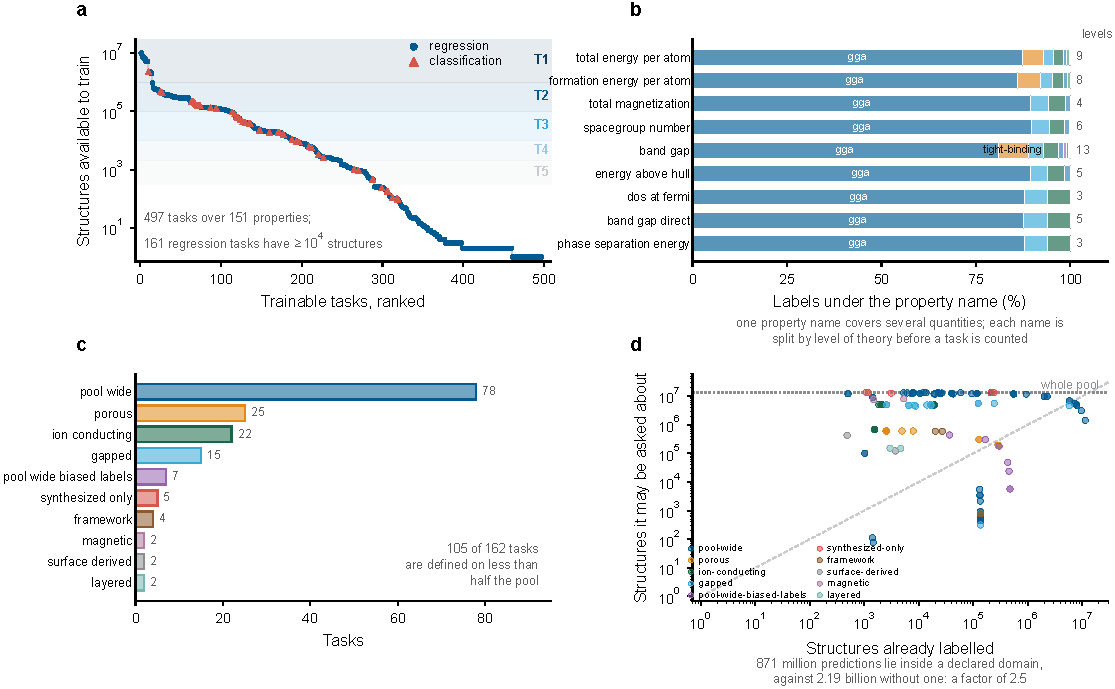
\includegraphics[width=0.99\textwidth]{figs/fig4_completion.pdf}
  \caption{\textbf{What the corpus offers a learned completion of the property
  layer.}
  \textbf{a},~How the registered properties become separable learning tasks and
  then realised training sets. The arrow marks the one stage that multiplies
  rather than filters, splitting a property name by level of theory.
  \textbf{b},~Composition of the most widely covered properties by level of
  theory, as a fraction of the labels filed under each property name. The figure
  at the right gives the number of distinct levels.
  \textbf{c},~The constructed training sets by declared applicability domain, the
  set of structures for which the property is defined at all.
  \textbf{d},~For each training set, the crystals already labelled against the
  crystals the task may legitimately be asked about once its domain is enforced.
  The dotted line marks the whole pool and the dashed diagonal marks parity.
  Panels reporting the trained models are added when their held-out numbers
  exist.}
  \label{fig:completion}
\end{figure}

A census of the database establishes how much is actually trainable
(Fig.~\ref{fig:completion}a). The unit that matters is not the property but the
property at one level of theory, because a name such as band gap covers several
different physical quantities that a model cannot distinguish from structure
alone. Split that way, the 151 populated properties yield 513 candidate tasks,
set against the tens that existing property-prediction and stability benchmarks
provide \cite{dunn2020benchmarking,riebesell2025framework}. Of
these, 165 regression tasks have at least $10^4$ crystals to train on, 100 have at
least $10^5$, and 13 have at least $10^6$. Constructing the training sets under a
default policy that keeps the largest level of theory per property produced 176
sets covering 116 properties and 93{,}864{,}594 labels, each with a
chemistry-aware train, validation and test split.

The four constraints are each a direct consequence of the integration reported
above. The first is that a property name is not a label definition
(Fig.~\ref{fig:completion}b).
Band gap carries 15 distinct levels of theory, of which the semilocal group holds
83\% and no other reaches 5\%. The systematic offsets between them
are of order 1~eV, which a model cannot infer from the structure and would
instead learn as a proxy for which database supplied the row. The second is that
some quantities are condition-dependent rather than multiply determined: carbon
dioxide uptake is reported at several distinct grand-canonical conditions, so a
material legitimately carries several different correct values and taking their
median produces a number that is not any physical quantity. Neither the level of
theory nor the condition is resolved away, and neither is the cross-source spread
of Section~\ref{sec:inherits}: across the training sets, 5{,}856{,}861 crystals
carry labels from two or more databases, and that spread is kept beside the
resolved value so that it can weight the loss rather than being averaged into
it.

The third is that the data cannot be split at random. The same compound
recurs in the pool under different accession numbers, so a random split places
identical chemistry in training and test, and the resulting scores are optimistic
in exactly the regime that matters, since the crystals a completion is wanted for
are the ones whose chemistry the training set never saw. Holding out whole
chemical systems is the right default, but it degenerates on the enumerated
libraries, where an entire task can occupy a single chemical system and a
chemistry-level holdout leaves the validation and test folds empty. The split
rule falls back for those tasks and records which level it used
(Supplementary Note~\ref{si-note:census}).

The fourth is that the completion has a domain (Fig.~\ref{fig:completion}c,d).
Carbon dioxide uptake is a grand-canonical adsorption quantity: it is not zero for a
dense intermetallic, it is undefined, because the simulation cell has nowhere to
insert a molecule. Of the 176 training sets, 63 draw more than 90\% of their
labels from a single material family (Fig.~\ref{fig:completion}c). Enforcing
their declared domains changes the size of the completion problem substantially: 109 of
the 176 tasks are defined on less than half the pool, and the number of
predictions that lie inside a declared domain is 1{,}105{,}593{,}143 rather than
the 2.57 billion that asking every task about every crystal would produce, a
factor of 2.3. The difference is not a loss of coverage. It is the removal of numbers
that would have looked like data. Plotting what a task may be asked about against
what it already knows separates the two situations that matter
(Fig.~\ref{fig:completion}d): a task lying far above the diagonal has the most to
gain, because its domain is large and its labels are few, while a task lying to
the right and low is one whose domain is already nearly labelled and where a
model has little left to add.

One dependency in that structure is worth stating because it closes the loop with
Section~\ref{sec:index}. Twenty-one of the tasks are gated on a property the
database does not yet hold: whether a crystal has a gap, or whether it is
magnetically ordered, is unknown for 108{,}246{,}933 structure-task pairs, so
their admissibility can only be decided once the corresponding tier-1 models have
run.
The completion therefore proceeds in stages, and each stage enlarges the domain
over which the next one is defined, in the same way that each admitted structure
enlarged the substrate against which the next database was matched.

What such a completion would settle is worth stating before it is attempted,
because it is the reason the corpus was assembled rather than merely enlarged.
Searching the known set for a material that already has the property wanted does
not require that the property have been computed, because a surrogate model can
rank crystals nobody has evaluated, and that is how such campaigns are run. What
is bounded is the pool over which the ranking is taken. A campaign screens the
repository it loaded, and Section~\ref{sec:inherits} sets both what any single
repository can offer as training signal and how far its labels can be trusted
where a second source exists. Running the completion over the whole corpus, within the
domains of Fig.~\ref{fig:completion}c,d, changes both terms at once: the pool
becomes the deduplicated record rather than one provider's slice of it, and every
label carries the spread of the sources that reported it.

That is what measures a quantity the field has never had: how much of the known
record has been passed over for want of a calculation rather than for want of
merit. A large yield would mean that forward screening has been
operating far inside its own reach. A small one would mean the reach is nearly
exhausted and that further progress has to come from designing structures rather
than finding them. The same corpus serves that second route as well, since a
generative model needs exactly what it holds: structures deduplicated across the
whole known record, so that novelty is judged against everything published rather
than against one repository, and property labels that name the quantity they
denote, so that a model can be conditioned on a defined target. Which of the two
answers the completed layer gives is an empirical question, and it is the one the
next stage is built to decide.

\PENDINGGNN

\PENDINGCANDIDATES

\subsection{Judging the novelty claimed by inverse design}
\label{sec:novelty}

The record that bounds forward screening is also the reference inverse design
needs, and the point of this section is that a reported novelty fraction measures
that reference at least as much as it measures the model. A generative model
counts as new whatever is absent from the reference set it was given, so a
structure missing from one repository but held by another is counted as new; the
reference sets in current use are drawn from a handful of the largest
repositories \cite{ramlaoui2025lemat,betala2025lematgenbench}, and the three
assessments cited in the Introduction all turned on exactly that
\cite{cheetham2024artificial,juelsholt2026continued,szymanski2025baselines}.

Two distinct failures sit behind those three assessments, and the corpus
assembled here has already met both from the other direction. The first is a
criterion too permissive, counting a known prototype under a new decoration as a
new material. The second is a criterion that misses a match it should have made,
which is what happens when an ordered approximant is generated for a parent phase
that is disordered on one site. Section~\ref{sec:index} reports the first as
over-merging in the enumerated framework libraries, where a bonding-graph
fingerprint collapses more than $10^5$ distinct hypothetical frameworks onto a
few hundred pool materials, and Supplementary Note~\ref{si-note:fingerprint}
states the domain within which that fingerprint is valid. Both are failures of the criterion rather than of the generator, and no published
novelty figure states which criterion produced it. What this record offers the
route is therefore not a better score but a reference that can be named: the
resolved corpus rather than a few of its largest members, and a matching rule
whose domain of validity is stated rather than assumed.

\PENDINGNOVELTY

\FloatBarrier
